
% Inbuilt themes in beamer
\documentclass[aspectratio=169]{beamer}
\usepackage{graphicx}
\usepackage{hyperref}
% Theme choice:
\usetheme{CambridgeUS}

% Title page details: 
\title{Probability and Statistics Review \\
        \large Econometrics discussion section 1} 
\author{John Green}
\date{Spring 2025}


\begin{document}

% Title page
\begin{frame}
    \titlepage 
\end{frame}

% housekeeping
\begin{frame}{Housekeeping}
    \begin{itemize}
        \item Introductions: name, major, thoughts about econometrics
        \item For now, office hour in Brody Cafe, Tuesdays, 3-4PM
        \begin{itemize}
            \item May change to Wyman Park 601A
            \item Timing poll: \href{bit.ly/metricsOH}{bit.ly/metricsOH}
        \end{itemize}
        \item What will we do in sections?
        \begin{itemize}
            \item Cover important topics
            \item Practice problems
            \item Stata practice
            \item Slides and resources in GitHub repo: \href{github.com/JohnRGreen/EconometricsSpring25}{github.com/JohnRGreen/EconometricsSpring25}
        \end{itemize}
        \item Sign in for attendance each week
    \end{itemize}
\end{frame}

% Outline frame
\begin{frame}{Recap}
    What have we covered so far?
    \begin{itemize}
        \item Review of probability and statistics (Stock \& Watson chapters 2 and 3)
        \item Random variables and their first 2 moments
        \item Marginal, joint and conditional distributions
        \item Independence
        \item Covariance and correlation
        \item Law of Iterated Expectations
    \end{itemize}
\end{frame}

\begin{frame}{Recap}
    Still to come (probably):
    \begin{itemize}
        \item Normal, Fisher (F), $\chi^2$ distributions      
        \item LLN and CLT
        \item Estimators and their properties: consistency, unbiasedness, normal approximation
        \item One variable t-test
        \item Two variable t-test
    \end{itemize}
\end{frame}

\begin{frame}{Random variables}
    \begin{itemize}
        \item A random variable is a \textit{function} from a space of possible outcomes to (usually) some subset of real numbers.
        \item May be discrete or continuous
        \item Roll two dice and add up the numbers (discrete)
            \begin{itemize}
                \item Sample space is all the possible rolls of the two dice (how many?)
                \item Outcome space is all the possible sums of those rolls (how many?)
                \item The sum is a random variable
            \end{itemize}
        \item Height of a person (continuous, but bounded)
            \begin{itemize}
                \item Sample space is all people; might think about characterizing them by some covariates such as weight, age, etc.
                \item Outcome space is all possible heights (what would this be?)
            \end{itemize}
        \item Thinking about probability is different for discrete and continuous cases
    \end{itemize}
\end{frame}

\begin{frame}
    \centering
    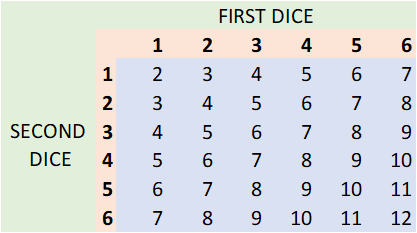
\includegraphics[width = 0.5\textwidth,keepaspectratio]{dice.png}
\end{frame}

\begin{frame}{Mean}
    \begin{itemize}
        \item The first moment of a random variable is its mean, aka average or expected value
        \item What is the mean value of the result from rolling one die?
        \item What is the mean value of the sum of rolling both dice?
    \end{itemize}
\end{frame}

\begin{frame}{Mean}
    \begin{itemize}
        \item The first moment of a random variable is its mean, aka average, aka expected value
        \item What is the mean value of the result from rolling one die?
        \begin{itemize}
            \item $E[X] = \frac{1}{6} \times 1 + \frac{1}{6} \times 2 + \frac{1}{6} \times 3 + \frac{1}{6} \times 4 + \frac{1}{6} \times 5 + \frac{1}{6} \times 6 = 3.5$
        \end{itemize}
        \item What is the mean value of the sum of rolling both dice?
        \begin{itemize}
            \item $E[X] = \frac{1}{36} \times 2 + \frac{2}{36} \times 3 + \frac{3}{36} \times 4 + \frac{4}{36} \times 5 + \frac{5}{36} \times 6 + \frac{6}{36} \times 7 + \frac{5}{36} \times 8 + \frac{4}{36} \times 9 + \frac{3}{36} \times 10 + \frac{2}{36} \times 11 + \frac{1}{36} \times 12 = 7$
            \item (Could also write out using $\frac{1}{36}$ weight everywhere but easier to consolidate terms)
        \end{itemize}
    \end{itemize}
\end{frame}

\begin{frame}{Variance}
    \begin{itemize}
        \item The second moment of a random variable is its variance
        \begin{itemize}
            \item Think of this as the mean distance from the mean: it measures the spread of our data
            \item $Var(X) = E \left[ (X - E[X])^2 \right] $
            \item Why do we need to square the spread?
        \end{itemize}
        \item What is the variance of rolling one die?
        \item What is the variance of the sum of rolling both dice?
    \end{itemize}
\end{frame}

\begin{frame}{Variance}
    \begin{itemize}
        \item The second moment of a random variable is its variance
        \begin{itemize}
            \item Think of this as the mean distance from the mean: it measures the spread of our data
            \item $Var(X) = E \left[ (X - E[X])^2 \right] $
            \item Why do we need to square the spread?
        \end{itemize}
        \item What is the variance of rolling one die?
        \begin{itemize}
            \item $Var(X) = \frac{1}{6} \times (1 - 3.5)^2 + \frac{1}{6} \times (2 - 3.5)^2 + \dots + \frac{1}{6} \times (6 - 3.5)^2 = \frac{35}{12} \approx 2.92$
        \end{itemize}
        \item Similar idea for the sum of 2 dice.
        \item Often we will work with the \textit{standard deviation} which is the square of the variance since the units are more interpretable.
    \end{itemize}
\end{frame}

\begin{frame}{Higher moments}
    \begin{itemize}
        \item Third moment is \textit{skewness} and tells us how symmetric our distribution is
        \begin{itemize}
            \item What is the skewness of our example?
        \end{itemize}
        \item Fourth moment is the \textit{kurtosis} which measures the mass of the tails
        \begin{itemize}
            \item Gives us an idea of the likelihood of large values
        \end{itemize}
    \end{itemize}
\end{frame}

\begin{frame}{Covariance}
    \begin{itemize}
        \item The covariance of two random variables tells us the strength of their \textit{linear} (careful!) relationship
        \item If two random variables are independent, covariance is 0 (though the reverse is not true)
        \begin{itemize}
            \item What is the covariance in our example?
        \end{itemize}
        \item Often we will look at the \textit{correlation} instead of the covariance, $\frac{cov(X,Y)}{(var(X)var(Y))^{1/2}}$
        \begin{itemize}
            \item Unlike covariance, correlation is scaled between -1 and 1 and so is easily interpretable
        \end{itemize}
    \end{itemize}
\end{frame}

\begin{frame}{Rules on joint distributions}
        \begin{itemize}
            \item If two variables are independent, $P(X=x,Y=y) = P(X=x)*P(Y=y)$
            \item Conditional probability: $P(X=x|Y=y) = \frac{P(X=x,Y=y)}{P(Y=y)}$
            \begin{itemize}
                \item What happens if the events are independent?
            \end{itemize}
            \item Law of iterated expectations says the mean of $Y$ can be written as a weighted average of the mean of $Y|X$: $E[Y] = E[E[Y|X=x]]$
            \begin{itemize}
                \item $E[Y] = \sum_x E[Y|X=x]P(X=x)$ in discrete case
                \item $E[Y] = \int_x E[Y|X=x]f_X(x)dx$ for continuous case
            \end{itemize}
            \item Other topics in textbook: Bayes' law, law of total probability, etc.
        \end{itemize}
\end{frame}

\begin{frame}{Second example}
    \begin{itemize}
        \item New example: 
        \begin{itemize}
            \item Roll the first dice
            \item If first roll $\geq 4$ then we roll the second die and observe its value
            \item If first roll $\leq 3$ then the second value is simply set to 1
        \end{itemize}
        \item What is the joint probability distribution?
        \item What is the covariance of the 2 rolls?
        \item What is the correlation?
        \item What is the marginal distribution of the two r.v.? What is the first moment of each?
    \end{itemize}
\end{frame}

\begin{frame}
    \centering
    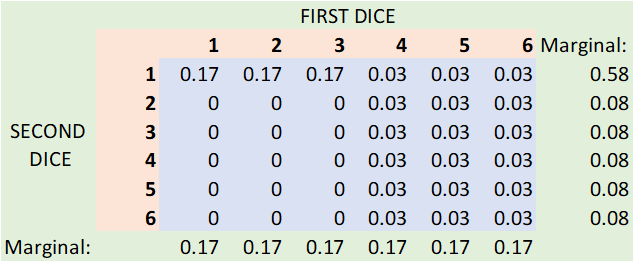
\includegraphics[width = 1\textwidth,keepaspectratio]{marginal.png}
\end{frame}

\begin{frame}{Second example}
    \begin{itemize}
        \item New example: 
        \begin{itemize}
            \item Roll the first dice
            \item If first roll $\geq 4$ then we roll the second die and observe its value
            \item If first roll $\leq 3$ then the second value is simply set to 1
        \end{itemize}
        \item What is the marginal distribution of the two r.v.? What are the first two moments of each? $E[X_1] = 3.5$, $var(X_1) = 2.92$, $E[X_2] = 2.25$, $var(X_1) = 3.02$
        \item What is the covariance of the 2 rolls? $cov(X_1,X_2) = 1.875$
        \item What is the correlation? $corr(X_1,X_2) = \rho_{X_1,X_2} = 0.63$
    \end{itemize}
\end{frame}

\begin{frame}{Normal distribution}
    \begin{itemize}
        \item Two parameters: mean $\mu$ and variance $\sigma^2$
        \begin{itemize}
            \item $\mu$ tells us about the location of the distribution (where is it centered?)
            \item $\sigma$ tells us about the shape of the distribution (what is the spread? what do the tails look like?)
        \end{itemize}
        \item We can \textit{standardize} a normal random variable X:
        \begin{itemize}
            \item $Z = \frac{X-\mu}{\sigma}$ so $Z \sim N(0,1)$
            \item Careful to divide by standard deviation and not by variance!
        \end{itemize}
        \item This will be helpful in hypothesis testing because we can consider how unlikely a given value $z$ is to be drawn from a N(0,1) distribution
    \end{itemize}
\end{frame}

\begin{frame}{Estimation}
    \begin{itemize}
        \item We will often be interested in estimating the mean of a distribution
        \item Example: wait time in Brody Cafe
        \item Natural estimator is a sample mean:
        \begin{itemize}
            \item Take a survey of people as they walk out of Brody and ask how long they waited
            \item Average the responses
        \end{itemize}
        \item Sample mean $\bar{Y}$ is a random variable since we taking a random sample and thus $\bar{Y}$ has a sampling distribution
        \begin{itemize}
            \item What can we say about it?
        \end{itemize}
    \end{itemize}
\end{frame}

\begin{frame}{Law of Large Numbers}
    \begin{itemize}
        \item $E[\bar{Y}] = \mu_Y$ 
        \item This means that $\bar{Y}$ is an \textit{unbiased} estimator of $\mu_Y$
        \item As our sample size grows, the sample mean will converge to the true mean
        \item $var(\bar{Y}) = \frac{\sigma_Y^2}{n}$ so that the variance of our estimator is decreasing as our sample gets larger
        \item So as our sample size grows, the sample mean will converge to the true mean: $\bar{Y}$ is a \textit{consistent} estimator of $\mu_Y$ (LLN)
    \end{itemize}
\end{frame}

\begin{frame}
    \centering
    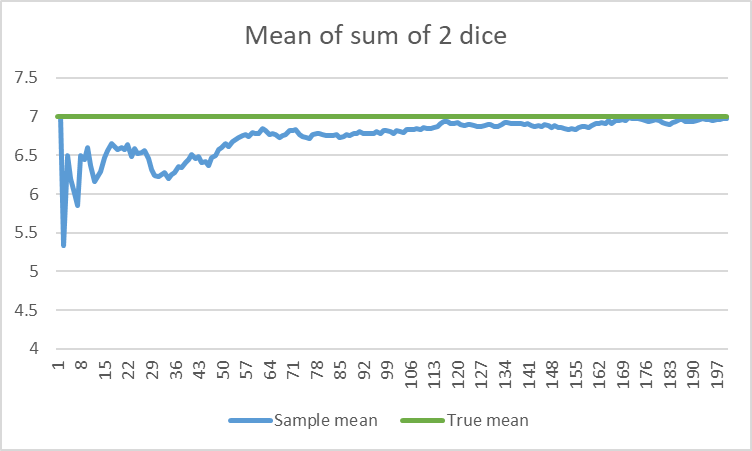
\includegraphics[width = .8\textwidth,keepaspectratio]{LLN.png}
\end{frame}

\begin{frame}{Central Limit Theorem}
    \begin{itemize}
        \item Even better: as $n \to \infty$, $\bar{Y}$ becomes normal ie $\bar{Y} \sim N(\mu_Y,\frac{\sigma_Y^2}{n})$
        \item This means that we can use the normal distribution to make inferences about the sample mean
        \item To make it easy, we can standardize the sample mean: $Z = \frac{\bar{Y} - \mu_Y}{\sigma_Y/\sqrt{n}} \sim N(0,1)$
        \item We will use the sample variance as an estimator for the population variance, just like we do for mean (but we will need to correct a small bias)
    \end{itemize}
\end{frame}

\begin{frame}{Hypothesis testing}
    \begin{itemize}
        \item We can use the normal approximation to perform a \textit{hypothesis test}
        \begin{itemize}
            \item One-sided or two-sided
        \end{itemize}
        \item Intuition: assuming the true mean is some value $\mu_{Y,0}$, how likely is it that we would observe the sample mean $\bar{Y}$?
        \begin{itemize}
            \item If it is ``very'' unlikely, we will reject the null
            \item If it is ``reasonably likely'' then we fail to reject the null
        \end{itemize}
        \item p-value: probability of a test statistic at least as unlikely as the one you observe (under the null)
    \end{itemize}
\end{frame}

\begin{frame}{Some other terminology}
    \begin{itemize}
        \item \textbf{Type-1 error}: reject a true null hypothesis
        \begin{itemize}
            \item \textbf{Size} is probability of a type-1 error
        \end{itemize}
        \item \textbf{Type-2 error}: fail to reject a false hypothesis
        \begin{itemize}
            \item \textbf{Power} is probability of a type-2 error
        \end{itemize}
        \item Which of these two mistakes is worse?
        \item What is the relationship between the size and the power?
    \end{itemize}
\end{frame}

\begin{frame}
    \centering
    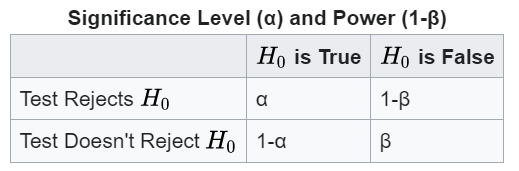
\includegraphics[width = .6\textwidth,keepaspectratio]{size_and_power.png}
\end{frame}

\begin{frame}{Calculating p-value}
    \begin{itemize}
        \item So, the \textbf{p-value} tells us how unlikely the null hypothesis is:
        \begin{itemize}
            \item  $P_{H_0}(|\frac{\bar{Y} - \mu_{Y,0}}{\sigma_Y/\sqrt{n}}|\geq |\frac{\bar{Y}_{data} - \mu_{Y,0}}{\sigma_Y/\sqrt{n}}|)$
            \item RHS is just a number! LHS is RV with known distribution under null
            \item CLT tells us this \textbf{t-statistic} is N(0,1) so probability in tails is easy to look up
        \end{itemize}
        \item If observed t-statistic is very large or very small, then p-value is very small and we reject the null
        \begin{itemize}
            \item If the null had been true, it is very unlikely that we would have observed the t-statistic
        \end{itemize}
    \end{itemize}
\end{frame}

\begin{frame}{Using pre-set significance level}
    \begin{itemize}
        \item Alternatively, we can decide that we want to do a test at a given significance $\alpha$ and find the value such that the sum in the tails (or tail) is $\alpha$
        \item Eg if $\alpha=0.05$, then our cutoff points are $(-1.96,1.96)$
        \item If our t-statistic is outside of these bounds, we reject the null because it was very unlikely
        \item This is always less-informative than a p-value; but may be more rigorous to pre-set our rejection region
        \item We can also construct a confidence interval for $\mu_X$ based on our data, eg $\bar{X} \pm 1.96 \frac{\sigma_X}{\sqrt{n}}$
        \begin{itemize}
            \item This is the set of all possible $\mu_X$ values which would not be rejected by a two-sided t-test with $\alpha=0.05$
        \end{itemize}
    \end{itemize}
\end{frame}

\begin{frame}{Hypothesis about difference in means}
    \begin{itemize}
        \item What if we want to perform a hypothesis on the difference in means between two random variables?
        \item Simple: combine them to one!
        \begin{itemize}
            \item $X_3 = \bar{X}_1 - \bar{X}_2$
            \item This is just a difference of two normal random variables so we can use the normal approximation, t-statistic is just $\frac{\bar{X}_1 - \bar{X}_2}{\sqrt{\frac{\sigma_1^2}{n_1} + \frac{\sigma_2^2}{n_2}}}$
        \end{itemize}
        \item What if we want to test hypothesis that the difference is 2?
    \end{itemize}
\end{frame}

\end{document}